This section show and discuss the results obtianed with the simulation described in section \ref{subsec:SourceShapeSimulation}, the objective of which is to find the radial thick of the simulated tritium source that reduce the comsuming time and computing resources used in the simulations. 

First, the initial energy of the simulated tritium events are verified. For this task, the energy distribution of the simulated tritium electrons is obtained, shown in figure \ref{subfig:EnergyDistributionTritiumSource}, and compared with that obtained in the reference \cite{TritiumEmissionSpectrum}. As can be checked, there is a good agreement between both.

In addition, a spectrum of the initial energy of tritium electrons that are capable of reaching the fiber and depositing energy are shown in Figure \ref{subfig:EnergySpectrumEventsDetectedandNonDetected}, red histogram, which is compared to the energy distribution of all simulated tritium events, blue histogram. A shift to the right side in the red histogram is observed, creating a peak centred at $10~\keV$. This shift occurs mainly because the lower energy tritium electrons don't have enough energy to reach the fiber and overcome the water-fiber interface, producing a non-detected tritium event.

\begin{figure}[h]
 \centering
  \subfloat[Energy distribution of tritium decays simulated]{
   \label{subfig:EnergyDistributionTritiumSource}
    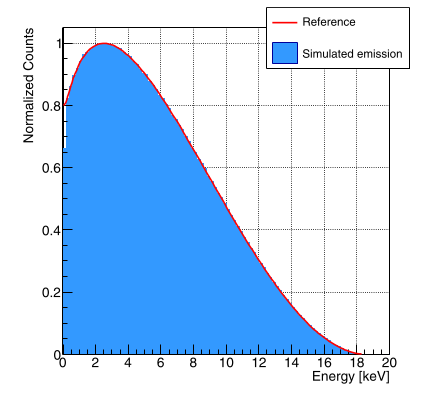
\includegraphics[width=0.5\textwidth]{8SimulationsResults/81TRITIUMDesign/811TritiumSourceOptimization/TritiumSourceEnergyDistribution.png}}
   %\newline
  \subfloat[]{
   \label{subfig:EnergySpectrumEventsDetectedandNonDetected}
    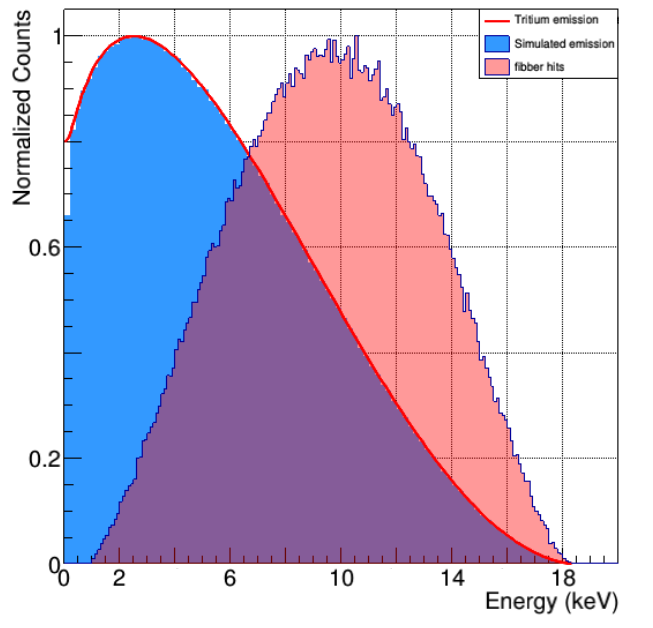
\includegraphics[width=0.5\textwidth]{8SimulationsResults/81TRITIUMDesign/811TritiumSourceOptimization/Source_Spectrum_yes_and_non_detected_events.png}}
 \caption{ Energy distribution of a) simulated tritium decays b) Initial energy of tritium decays that reach the scintillating fibers (red histogram) compared the all simulated tritium events (blue histogram) \cite{SimulationPaperCarlos}.
 \label{fig:TritiumSourceOptimization}}
\end{figure}

Regarding the radial thickness of the tritiated water source, Figure \ref{subfig:TransversalCutTritiumSource} shows a transversal cut of the $2~\mm$ scintillating fiber, yellow, the simulated tritium source $0.5~\mm$ thick around the fiber, green, and the tritium decays the electrons of which has deposited their energy in the scintillating fiber, red dots. Furthermore, the distribution of the radial distance between the position where tritium decays take place and the surface of the scintillating fiber are shown in figure \ref{subfig:DistanceDistributionTritiumSourceFiber}.

\begin{figure}[h]
 \centering
  \subfloat[]{
   \label{subfig:TransversalCutTritiumSource}
    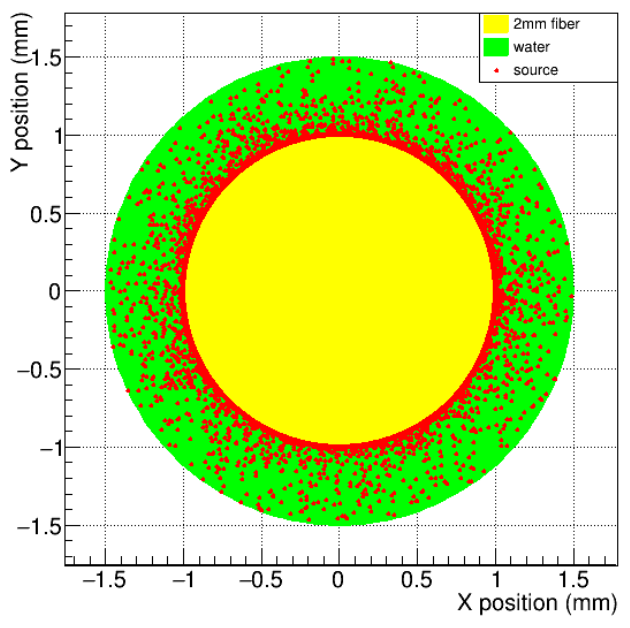
\includegraphics[width=0.5\textwidth]{8SimulationsResults/81TRITIUMDesign/811TritiumSourceOptimization/Source_Ring.png}}
   %\newline
  \subfloat[]{
   \label{subfig:DistanceDistributionTritiumSourceFiber}
    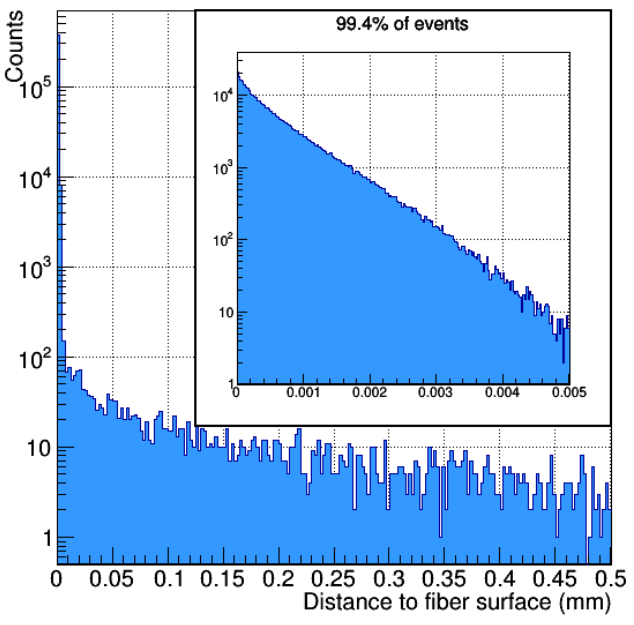
\includegraphics[width=0.5\textwidth]{8SimulationsResults/81TRITIUMDesign/811TritiumSourceOptimization/SourceDistance.png}}
 \caption{a)Transversal cut of simulated scintillating fiber (yellow) and tritium source (green) with various tritium decays (red dots) b) Distribution of the radial distance between the position where the tritium decay takes place and the surface of the scintillating fiber \cite{SimulationPaperCarlos}.}
 \label{fig:TritiumSourceSimulated}
\end{figure}	

As can be seen in both figures, most of the tritium decays that are detected occur in close proximity to the scintillating fiber.  A zoom is applied in the inset box of the Figure \ref{subfig:DistanceDistributionTritiumSourceFiber} for better viewing. The chosen thickness of the simulated tritium source is $5~\mu\meter$ since the $99.4\%$ of the events that are able to deposit energy in fibers are produced at least of this distance.